\documentclass{article}
\usepackage{graphicx}
\usepackage{amsmath}
\usepackage{hyperref}
\usepackage{listings}
\usepackage{xcolor}
\usepackage{hyperref}

\lstset{
    language=Python, % Change this to the language you are using
    basicstyle=\ttfamily\footnotesize,
    keywordstyle=\color{blue},
    stringstyle=\color{red},
    commentstyle=\color{green},
    numbers=left,
    numberstyle=\tiny\color{gray},
    stepnumber=1,
    numbersep=5pt,
    backgroundcolor=\color{lightgray},
    showspaces=false,
    showstringspaces=false,
    breaklines=true,
    frame=single,
    captionpos=b
}

\title{Classification of Vegetation Types Using Time Series Satellite Imagery - Sentinel-2}
\author{Filippo Giovagnini}

\begin{document}

\maketitle

\begin{abstract}
    This report presents the findings and methodologies used in the data analysis project titled "Classification of Vegetation Types Using Time Series Satellite Imagery - Sentinel-2". The aim of this project was to analyze time series satellite imagery data from Sentinel-2 to classify different vegetation types. Various data preprocessing techniques and analytical methods, including machine learning algorithms, were employed to ensure the accuracy and reliability of the results. The key findings highlight significant patterns and trends within the satellite imagery data, providing valuable information for environmental monitoring and decision-making.
\end{abstract}

\section{Introduction}
\label{sec:intro}
We first present some initial considerations that allowed for the implementation of several methods and then the selection of the most efficient one. First of all, it was observed that the problem in question falls into the category of classification problems. There is a certain number of vectors of length 46 (corresponding to the 46 images taken by the Sentinel-2 satellite) accompanied by a label that corresponds to the type of crop present in that geographic region. A preliminary consideration for selecting the appropriate model is the following. Since the dataset was obtained by randomly selecting pixels from the images taken by the satellite, there is no spatial information. This means that the relative position of the various pixels in the dataset cannot be exploited. One possibility, in fact, would have been to first use neural networks to recognize plots of land, thereby creating a sort of vocabulary, and then use a neural network to classify each recognized plot based on its temporal evolution. However, the work done in Garnot et al. (2019) is interesting but not applicable to this problem. Therefore, the focus shifts to studying methods that limit themselves to classification based on temporal evolution. The programming language that will be used in this work is Python. The computer on which the programs were run is a 2020 MacBook Pro (8-core CPU with 4 performance cores and 4 efficiency cores, 8-core GPU, 16-core Neural Engine).



\section{Preliminary Analysis and Data Preprocessing}
\subsection{Qualitative Analysis}

From now on, we will refer to a pixel as the geographic region represented by a single vector of dimension $(1,46)$, which in our case corresponds to an area of $64 m^2$.
The following table shows the occurrences of the various crops:
\begin{table}[htpb!]
\centering
\begin{tabular}{|l|c|}
\hline \text{Crop Number} & \text{Occurrences} \\
\hline 1 & 47696 \\
2 & 33204 \\
3 & 6524 \\
4 & 864 \\
5 & 7524 \\
6 & 18692 \\
7 & 9616 \\
8 & 12952 \\
9 & 30204 \\
10 & 2640 \\
12 & 4900 \\
13 & 412 \\
14 & 14020 \\
15 & 1272 \\
17 & 3692 \\
18 & 864 \\
19 & 3860 \\
20 & 488 \\
\hline
\end{tabular}
\end{table}

\begin{figure}[htpb!]
    \centering
    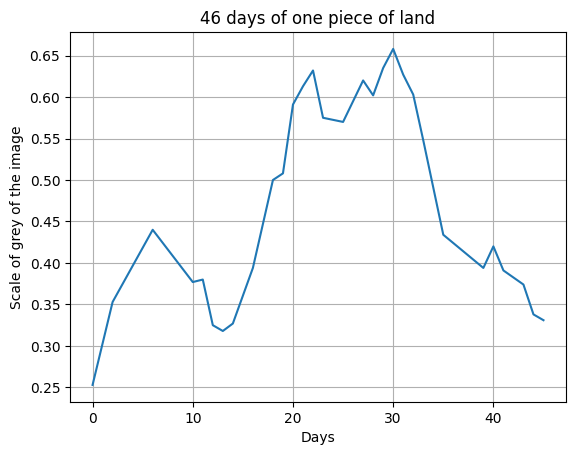
\includegraphics[width=0.5\textwidth]{output.png}
    \caption{Representation of a vector from the dataset.}
    \label{fig:visualization}
\end{figure}

The choice of the model was made by comparing the results obtained with the various models. The models that were tested are the following:
\begin{itemize}
    \item Convolutional Neural Network (CNN)
    \item Long Short-Term Memory (LSTM)
\end{itemize}

\section{Cross Validation of LSTM Model}

In order to find the best hyperparameters for the LSTM model, a grid search was performed. The following hyperparameters were tested:

\begin{lstlisting}[caption={Hyperparameters}, label={lst:example}]
    param_grid = {
    'input_dim': [46],
    'hidden_dim': [128, 256, 512],
    'layer_dim': [1, 2],
    'output_dim': [20],
    'seq_dim': [128],
    'lr': [0.001, 0.0005],
    'batch_size': [64, 128],
    'n_epochs': [100, 200],
    'patience': [10, 20]
    }
\end{lstlisting}

The best hyperparameters were found to be the following:

\[
    (46, 128, 1, 20, 128, 0.001, 64, 200, 20)
\]

The Cross Validatiion was performed ony in $n = 50000$ samples of the dataset. 


\section{Choice of the model}
\label{sec:model}

As the second gave a better accuracy, we decided to use the LSTM model. The model was trained using the Adam optimizer with a learning rate of $0.001$ and a batch size of $64$. The model was trained for $500$ epochs. The loss function used was the categorical Cross-Entropy.

\begin{figure}[htpb!]
    \centering
    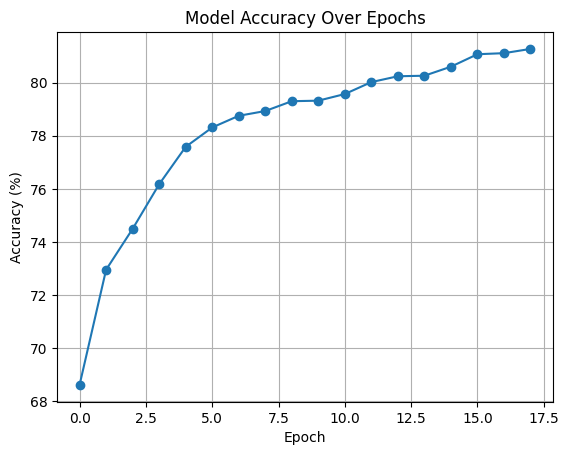
\includegraphics[width=0.5\textwidth]{accuracy.png}
    \caption{Accuracy of the LSTM model.}
    \label{fig:loss}
\end{figure}

\section{Results}
\label{sec:results}

It turns out that the accuracy of the LSTM model is $81.93$. The training time is also relatively low, as the model was trained in $23$ minutes. The model was trained on $199424$ samples of the dataset. You can find all the code used in \href{https://github.com/filippogiovagnini/sentinel-2_land_classification}{https://github.com/filippogiovagnini/sentinel-2\_land\_classification}.

\end{document}